\documentclass[a4j,8pt,twocolumn]{extarticle}

% ---------------

\usepackage{winf-paper}
\usepackage{amsmath}
\usepackage{amssymb}
\usepackage{ascmac}
\usepackage{latexsym}
\usepackage{ulem}
\usepackage[dvipdfmx]{graphicx}

% ---------------

%% 和文題目
\title{滞在ウォッチの複数コミュニティ間連携に向けた取り組み}

%% 和文著者
\author{外山瑠起 \qquad 亀田優作 \qquad 梶克彦}

%% 和文所属
\affiliation{愛知工業大学 情報科学部}







% ===== 所属が複数の場合 =====
%\author{情報 太郎\DAG{1} \qquad 情報 花子\DAG{1} \qquad 情報 次郎\DAG{2}}
%\affiliation{\DAG{1}情報大学情報学部 \qquad \DAG{2}情報大学大学院情報学研究科}
%\eauthor{Taro Info\DAG{1} \qquad Hanako Info\DAG{1} \qquad Jiro Info\DAG{2}}
%\eaffiliation{%
%	\DAG{1} Faculty of Information, Information University\\
%	\DAG{2} Graduate School of Information, Information University
%}

\begin{document}

\maketitle
\thispagestyle{empty}	% 1ページ目のページ番号を表示しない
% ------------------------------------------------------------

\section{はじめに}
ここ数年コロナ禍において対面でのコミュニケーション機会が減少している.
ニッセイ基礎研究所は全国の 20 ~ 74 歳の男女を対象とした新型コロナの感染拡大前(2020 年1月頃)と比べた「家族や友人との対面でのコミュニケーション」の変化についてのインターネット調査\footnote[1]{https://www.nli-research.co.jp/report/detail/id=70465} を行った.
その結果,全体平均で「減少」が 22.7\%「やや減少」が 18.8\% 両方合わせた減少層は 41.5 \%となった.

人同士のコミュニケーション頻度が低下しているなら特定のコミュニティ内でも同じことが起きていると言える.
特定のコミュニティ内でのコミュニケーション頻度が低下しているなら複数のコミュニティ間でのコミュニケーション頻度はさらに落ちていると言える.
具体例をあげるとコミュニティが大学の研究室にあたり,複数のコミュニティ間というのは研究室同士の集合を指す.
このような例は学校,職場など複数のコミュニティがあるところで同じように存在しており同様の現象が起こっていると考えられる.
エン・ジャパン株式会社のインターネットアンケー ト \footnote[2]{Kcorp.en-japan.com/newsrelease/2020/24687.html} によると「コミュニケーションがうまく取れるかどうかは, 仕事に影響すると思いますか?」という問いに対して ”思う ”と回 答したのが 80 \%を記録している.
上記のアンケートからわかるようにコミュニケーション頻度の低下はコミュニティ及び複数コミュニティ間の活性化を阻害する可能性がある.


これを改善するために我々は在室情報に注目した.誰がどの部屋に滞在しているかという在室者情報は様々な利用が期待できる.目的とする人の居場所が分かればコミュニケーションの円滑化や共同作業を支援できる.部屋の混雑度合いを共有すれば三密対策として利用可能である. 今後のウィズコロナ時代にも,いつ・どの部屋に滞在していたかという記録は後日の接触確認が可能な情報として重要となる.

そこで我々は BLE ビーコンを用いた在室管理プラットフォーム「滞在ウォッチ」を提案する.本研究では利用者の負担軽減のために,在室者情報を BLEビーコンで受動的に記録する方法を採用した.
在室管理プラットフォームの概要を図 1 に示す.ビーコンを持った利用者が部屋に訪れると受信機が検知し,サーバに在室者情報を送信しデータベースに記録する.
データベースに保存された情報は独自に作成した API によって外部からの利用が可能である.APIによって退勤管理システムや在室状況可視化システム,部屋利用者の来訪促進システム,コミュニケーション促進システムなど様々な応用システムの構築ができる.

この滞在ウォッチを複数コミュニティに導入・運用可能な状態にした上で複数間コミュニティで活発にコミュニケーションが行われる仕組みの実現をするのが本研究の最終目標である.
各コミュニティにおける在室情報を利用し,ゲーミフィケーションやナッジといった行動変容を促す仕組みに基づいてコロナ禍においても適切な範囲内でコミュニティ間の交流が促進されるようなシステムの構築を目指す.
本論では滞在ウォッチを複数コミュニティで連携するための取り組みを述べる.

\begin{figure}[tbh]
    \centering
    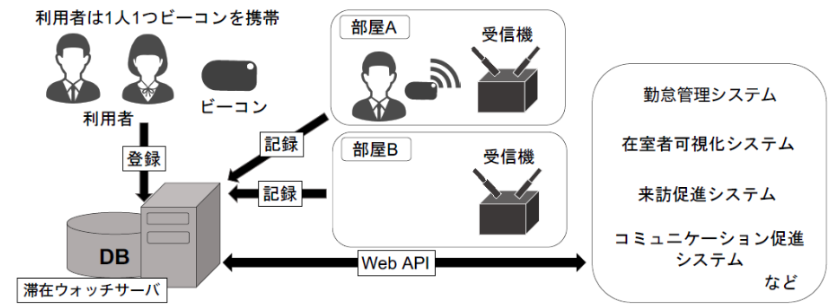
\includegraphics[width=8cm]{figure1.jpg}
    \caption{「滞在ウォッチ」の概要図}
    \label{multipleBPM}
\end{figure}

\section{関連研究}
在室状況提示システムを構築する際に入退室時刻の推定をするために過去その部屋に在室した時刻情報が必要である.在室した時刻情報を取得する方法はいくつか考えられる.在室者情報を取得する研究としてICカードを用いて在室者情報を能動的に記録する方法がある [1].この方法では在室者情報を確実に記録できるがICカードを用いて能動的に記録する必要があるので利用者への負担がかかってしまう.

また,顔画像を用いた入退場システムがある [2].このシステムはあらかじめ登録してある顔画像と入場者の顔画像を顔認証ソフトウェアによって比較し同一人物か判定している.このシステムはICカードよりも利用者の負担軽減につながるがコストがかかってしまう.

また,複数カメラを用いた 顔認証在室管理システムがある [3].各デスクの専用の識別器を作成し,カメラによってメンバを認識した場合に在室確認ができるというシステムである.識別器を作成する際に機械学習をする必要があり,学習の時間が必要である.またこのシステムでの学習後の識別率が65\%であり個人を特定するのに十分な精度とは言えない.

また,スマートフォンとビーコンを用いた出席管理システムがある [4].このシステムは個人の持つスマートフォンを受信機として,室内にビーコンを設置しビーコンの電波を受信したスマートフォンで利用者の位置を特定する.利用者の多くがスマートフォンを所持している点から運用コストが抑えられるがスマートフォンを所持していない人への対応やアプリケーション操作の手間がある.

\section{滞在ウォッチ}
本項では在室者情報を BLE ビーコンによって受動的に記録した情報を基に様々なシステムに応用可能なプラットフォーム「滞在ウォッチ」の概要について説明する.図1に示したようにまず部屋利用者1人ずつにビーコンを所持してもらう.使用するビーコンは株式会社フォーカスシステムズが販売するFCS1301[5]という小型ビーコンである.FCS1301は業務用の薄型ビーコンで用途として社員証や鍵などの貴重品につけて紛失防止や,徘徊者やペットの見守り支援などがある.そのため,個人が携帯するビーコンとして適している.また部屋利用者はビーコンを所持するだけなので,スマートフォンなどの別の機器を必要としないため負担が少ない.ビーコンを所持した部屋利用者が部屋を訪れると受信機がそれを検知しサーバに在室者情報を送信する.受信機は図2に示す Raspberry Pi[6]を使用する.Raspberry Piは低価格な機器のため導入コストを低く抑えられる.
\begin{figure}[tbh]
    \centering
    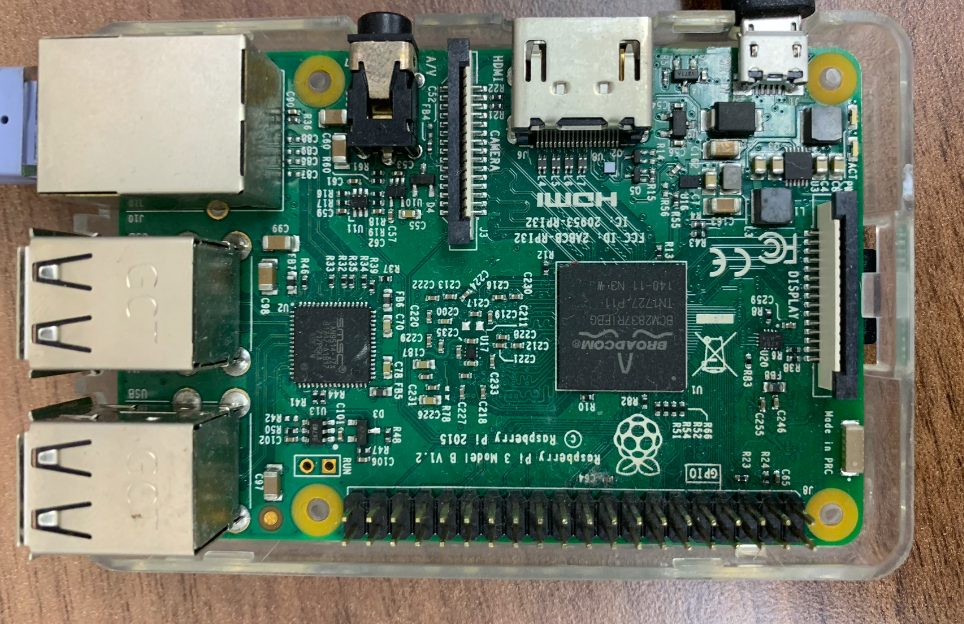
\includegraphics[width=8cm]{ras.jpg}
    \caption{Raspberry Pi}
    \label{multipleBPM}
\end{figure}

在室者の情報は,個人の現在の在室状況,過去の在室履歴,累計の在室時間などが Webページから参照可能である.過去の在室履歴には入室時刻と退室時刻が記録されている.在室者情報を 閲覧するのが部屋の管理者であった場合,閲覧方法が Webブラウザだけなど限られた状況であっても支障はない.しかし,本研究では利用者の在室者情報を他のシステムへ応用する.そのため データベースに保持されたデータは独自に作成した APIによって外部からの利用が可能である.

他のシステムへの応用例として出席管理システムがある.我が研究室ではミーティングの際に代表者が出席した人をエクセルシートに書き込み出席の有無を記録していた.この滞在ウォッチを基盤とした出席管理システムではミーティング時間にその人が研究室内に滞在していたかを判定・記録する.代表者はWebページから出席登録ボタンを押すことでエクセルシートにその記録が書き込まれる.代表者が能動的な記録を必要としないので負担軽減につながっている.

% ------------------------------------------------------------
\section{複数コミュニティへの拡張に向けた取り組み}
滞在ウォッチの研究室内運用を通して複数の問題が存在しており,本項ではその改善を目指した取り組みを説明する


% ------------------------------------------------------------

\subsection{受信機データの精度向上}
隣接した部屋の在室判定精度向上と判定誤検知を減らすために受信機データの精度向上を行った.
以前は1度のスキャン終了後にデータを送信する方法を使用していたがビーコンの発進間隔の都合上,全てのビーコンをスキャンするのが難しい場合が存在した.
そこで部屋ごとに設置された受信機が一定時間 周辺機器のスキャンを行う.
その後スキャンを数回繰り返しスキャンされたUUIDごとのRSSIの合計値をスキャンされた回数で割り平均化して送る形を採用した.
ここでの RSSI の合計値とスキャンされた回数は受信機のデータベースに保存しておりサーバ側にデータを送信する際に全てのデータをクリアする.
毎回送信されたデータをサーバ側で複数回受け取りその値を平均化するという手法もあったが処理の複雑化,サーバ側の過剰な負荷の懸念があったためこの方法を採用した.



\subsection{コミュニティ間の在室者情報の共有}

複数コミュニティでの運用を考えた場合,最低でもコミュニティごとに部屋が 1 つ以上は存在するため複数の部屋の入室・退室・継続して在室・移動を判定する必要である.過去のシステムでは単一の部屋の在室状況しか把握できなかったためシステムの再設計・再実装を行った.
受信機側からは図3に示すデータ形式でHTTPのPOSTメソッドを使って送信する.
\begin{figure}[tbh]
    \centering
    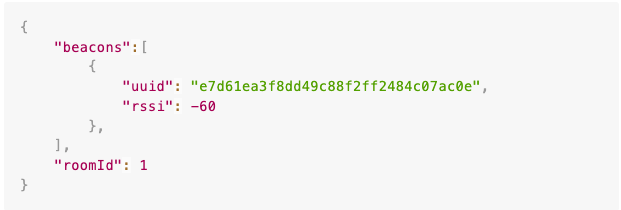
\includegraphics[width=8cm]{data.jpg}
    \caption{受信器が送信するデータ}
    \label{multipleBPM}
\end{figure}

送信されたデータはサーバ側で受け取りUUIDとROOMIDを使ってデータベースからユーザ情報と部屋情報を参照する.
在室しているかどうかを把握するためにデータベースに図4に示すようなStayersテーブルを使用する.
\begin{figure}[tbh]
    \centering
    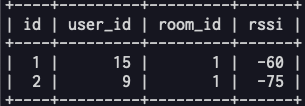
\includegraphics[width=8cm]{stayers.jpg}
    \caption{Stayersテーブル}
    \label{multipleBPM}
\end{figure}
ユーザの行動としては入室,退室,在室を継続,別の部屋への移動の4パターンが考えられる.送信されたデータからユーザを特定そのユーザがStayersテーブルに存在しない場合ユーザが入室したとする.送信されたデータの中にStayersテーブルと同じ部屋で同じユーザが存在しない場合ユーザが退室したとする.Stayersテーブルにユーザが存在しており送信されたデータにもユーザが存在するかつ同じ部屋の場合はユーザが継続して部屋に在室していると判断する.Stayersテーブルにユーザが存在しており送信されたデータにもユーザが存在するが部屋が異なりかつ送信されたRSSIの値がStayersテーブルのユーザのRSSIよりも値が小さい場合部屋を移動したと判断する.


\subsection{Web ページ閲覧の制限と管理}
 在室情報はプライバシーに関わるものであるため複数間コミュニティで適切に扱う必要がある.滞在ウォッチ利用ユーザの中には自身の在室情報を滞在ウォッチを利用しているユーザにのみ公開しても良い人,同じコミュニティに所属している人にのみ公開しても良い人,そもそも情報を公開するが嫌だという人,様々なユーザが想定される.
 そこで Web ページ閲覧者の制限とユーザによる情報公開範囲の変更を行うためにログイン機能の実装を行った.この場合の制限は管理者が登録したユーザのみ閲覧できるものである.ログイン機能には Firebase Authentication,OAuth2.0,Googleアカウント を使用した認証システムを使用している.ユーザ認証システムを独自で実装するという方法もあるが,パスワードのハッシュ化,ハッシュ化に利用している関数の脆弱性,フォームの改竄リスク等,気をつけなければいけないセキュリティリスクがいくつか存在する.Firebase Authentication を利用した実装ならばそれらのリスクを排除できる.

利用ユーザはGoogleアカウントを用いた認証を行うことで新しくIDとPASSWORDを作ることなくページ閲覧が可能である.まずWeb ページ上のログインボタンを押すと Firebase SDK を利用してリダイレクトを行い図5に示すように Google 認証画面に移動する.ここでユーザが許可すると Google の認可サーバがアクセストークンを発行するための認可コードを発行, Web ページにリダイレクトする.リダイレクト時に付与された認可コードを認可サーバに渡すことでアクセストークンを取得する.
次に Web ページから認証 API に対してリクエストを行う.このリクエストはリクエストを送ったユーザが管理者が登録したユーザであるかを確認するために行う.
Webページ側は取得したアクセストークンをHTTP のリクエストヘッダーに付与してリクエストを送る.
認証 API 側はヘッダーからトークンを取得 Firebase Admin SDK を利用してクライアントから送られてきたトークンが正しいユーザのものであるかの検証を行う.
トークン情報が正しくない場合はサーバ側は ステータスコード401,
トークン情報は正しいがトークンから得られるメールアドレスがデータベースに存在しない場合は ステータスコード 403,トークン情報が正しくトークンから得られるメールアドレスが存在する場合は ステータスコード 200 を返す.
Web ページ側は ステータスコード によって適切なコンテンツの表示を切り替えを行っている.

\begin{figure}[tbh]
    \centering
    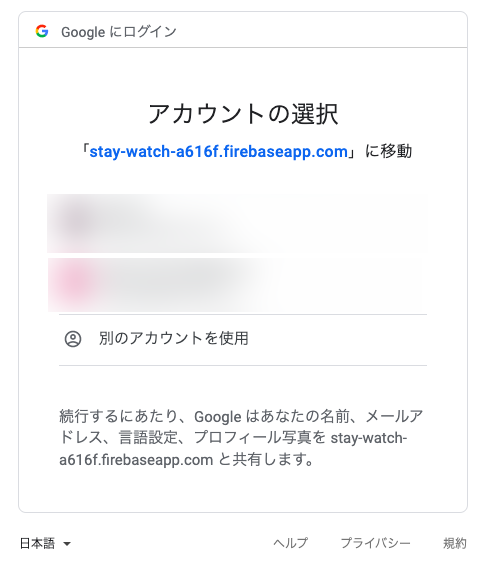
\includegraphics[width=8cm]{googleLogin.jpg}
    \caption{Google認証画面}
    \label{multipleBPM}
\end{figure}

管理者側はユーザの登録を行う.図6に示すように登録フォームでユーザネームと Gmail アドレス,ユーザロールを入力する.
ユーザネームは Web ページで表示される名前である,Gmail アドレスは閲覧を許可する Google アカウントに紐つくメールアドレス,ユーザロールは登録者の権限レベルを表す.
管理者が登録すると該当ユーザのメールアドレスに対して登録が完了したメールが送信される.
メールを受け取ったユーザはログインするとWebページの閲覧が可能となる.
\begin{figure}[tbh]
    \centering
    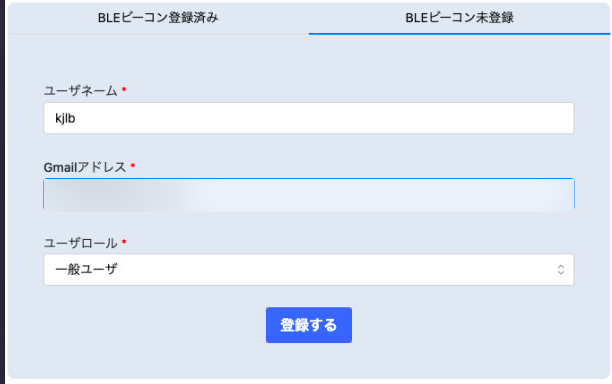
\includegraphics[width=8cm]{admin.jpg}
    \caption{管理者画面}
    \label{multipleBPM}
\end{figure}


\subsection{BLEビーコンのアプリケーション化による可用性向上}
BLEビーコンのアプリケーション化による可用性向上
ユーザの利便性向上のために,BLEビーコンのアプリケーション化をした.
BLEビーコンの導入は容易だが,運用上の諸問題がある.在室判定精度の向上のために,ビーコンは常に動作する必要がある.
しかしBLEビーコンのバッテリー残量の把握は専用のアプリケーションによる接続を要し,バッテリー切れに気が付かなかったユーザや,電池交換を手間に感じたユーザにバッテリー切れを起こしたビーコンが放置される状況が存在した.
これらの問題は,アプリケーション化に伴いハードウェア面,ソフトウェア面から改善がされた.
ハードウェアとして動作するスマートフォンはユーザが高頻度で状態を確認するため,バッテリー切れなど状況の判別が容易である.
また,スマートフォン自体の可用性を維持するために対策を講じるユーザが多く,ビーコンと比較してハードウェアとして可用性が維持されやすい.
ソフトウェア面では,図7に示す通りスマートフォンの通知領域に動作状況を可視化する.通知領域への表示はビーコンとしての動作と連携しており,アプリケーションの動作中は永続的に表示される.
よってアプリケーションが停止した場合もユーザによる判別が容易であるため,アプリケーション再起動によって可用性が維持されやすい.

\begin{figure}[tbh]
    \centering
    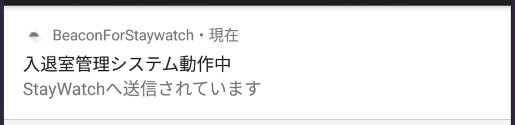
\includegraphics[width=8cm]{trans.jpg}
    \caption{通知領域による可視化}
    \label{multipleBPM}
\end{figure}



またバックグラウンド動作によってユーザ操作の負担を低減している.
既存のBLEビーコンの利点として正常に動作している限り,ユーザの操作が不要である点が挙げられる.
アプリケーション化に伴い,ユーザの操作が必要になったがそれを最小限に抑えるため,バックグラウンド動作による負担低減を行った.
ユーザの必要な操作は初回のみ必要なログイン処理とビーコン動作の切り替え処理のみである.ログイン処理ではFirebase Authenticationによって登録されたユーザか検証し,データベースからビーコンのデータを取得する.
ビーコン動作の切り替え処理はユーザの事情に応じた選択肢を提供する.在室情報のデータ可用性の観点からは常時のビーコン動作が望ましいが,同時にユーザの使用するスマートフォンのプライバシー性などへの配慮など倫理的課題が存在する.
それらの観点から図8に示すようにビーコン動作の停止が可能になる動作切り替え処理ボタンを提供する.
また,アプリケーション停止時に自動でビーコン動作の復帰が行えないため,ユーザが通知領域で動作していない状態を確認した場合,自らビーコンの動作を開始できる.


\begin{figure}[tbh]
    \centering
    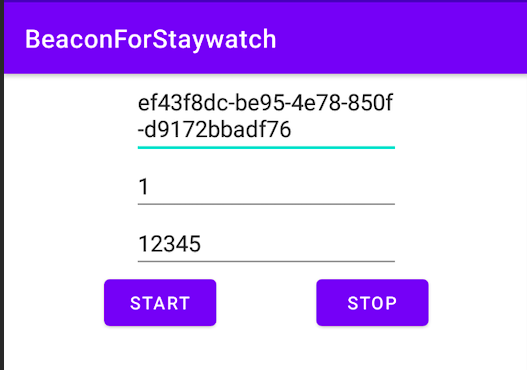
\includegraphics[width=8cm]{using.jpg}
    \caption{ビーコン動作切り替え画面}
    \label{multipleBPM}
\end{figure}


\subsection{BLEビーコンとスマートフォンのハイブリッド化に対応したシステム}
受信機側が4.4で述べたBLEビーコンのアプリケーションとBLEビーコンのどちらでも在室を検知できる仕組みを作成した.
従来の滞在ウォッチはBLEビーコンを各自が持ち歩きその情報をもとに部屋の判定を行っていた.
しかしこの方法は,専用アプリを使ってBLEビーコンのUUIDを設定する必要があるためヒューマンエラーが起きる可能性やコストが大きい問題がある.そのため他のコミュニティに導入を要請しても受け入れてもらえない可能性がある.
そこでBLEビーコンとスマートフォンの両方を使用してこの問題の解決を図った.
使用者のスマートフォンはBLEビーコンと同じUUIDを持つBLE機器として電波を発信する.スマートフォンを持っていればBLEビーコンを持っていなくても受信機は使用者が部屋に在室しているかを判定できる.スマートフォンがもつUUIDは管理者がメールアドレス登録済みの場合,アプリケーションのセットアップ時にサーバ側に問い合わせを行い,それに紐づいたUUIDを利用する.

このハイブリットシステムではユーザの負担を低減しつつ網羅的に在室情報の蓄積ができる.
ハイブリットシステムとしての運用はBLEビーコンとスマートフォンの両方をBLE機器として扱いお互いの利点を活かしている.
スマートフォンの電波を用いて在室推定する場合には,特別なアプリのインストールが必要となる.研究室内の学生などにはあらかじめインストールを依頼できるが,スマートフォンを持っていない一部の学生や学外から一時的に来訪する人に対するインストール依頼は難しい.一方BLEビーコンであれば警備室等で来訪時に渡すゲストカード等に付属させることが可能である.






% ------------------------------------------------------------
\section{おわりに}
本研究では BLE ビーコンを用いた在室管理プラットフォーム を提案した.「滞在ウォッチ」は BLE ビーコンによって受動的に 記録された在室履歴を API によって外部から利用できる在室管理プラットフォームである.
また在室管理プラットフォームを複数間のコミュニティで運用を目指すための構築を行った.
各コミュニティにおける在室情報を利用し,ゲーミフィケーションやナッジといった行動変容を促す仕組みに基づいてコロナ禍においても適切な範囲内でコミュニティ間の交流を促進するのが目的である.

今後の課題として現段階では1つのコミュニティでの運用しかされていないため,実際に複数のコミュニティに導入してもらい,運用を行う必要がある.運用後は,ユーザからの意見や得られたデータを元にシステムの改善を行う予定である.また現状のシステムではコミュニケーションを促進するような仕組みがないためその仕組みづくりを行いたい.















% ------------------------------------------------------------
\begin{thebibliography}{9}

\bibitem{KMST:2008}
藤原 仁貴, 村田 雄一, 堀 竜慈, 鈴木 俊吾, 志築 文太郎, 田中 二郎:メンバーの習慣を可視化する電子行方表とその評価, インタラクション 2010 論文集, SB18, p.1-4(2010).

\bibitem{HKS:1997}
西山 雄吾, 奥村 明俊, 半田 享, 星野 隆道, 津雲 淳, 高木 剛, 窪田 清仁:顔認証ソフトウェアを用いたチケット本人確認システム, 情報処理学会論文誌, Vol.78, No.1, p.493-494 (2013).

\bibitem{HKS:2019}
小林 祐貴, 田中 二郎:複数カメラの分散協調による顔認証在室管理システム, 第 81 回全国大会講演論文集, p.153-154(2019)

\bibitem{HKS:2016}
D. Deugo.,”Using Beacons for Attendance Tracking”, Frontiers in Education:CS and CE,FECS,p.155-161, (2016).

\bibitem{HKS:2022}
https://www.focus-s.com/focus- s/products/iot/blebeacon/fcs1301,(最 終 閲 覧 日:2022 年 10 月 22 日)

\bibitem{HKS:2022}
https://www.raspberrypi.org,(最終閲覧日:2022 年 10 月 22 日)






\end{thebibliography}




% ------------------------------------------------------------
\end{document}
